% !Mode:: "TeX:UTF-8"

\chapter{生成调度表}
\label{DLS-chapter-SSL}

% 路由策略、调度策略(抢占、非抢占)、任务分配

COSS 算法的下一步需要从 DAG 生成最终任务和消息的调度表,除了面对一般的 DAG 调度问题外,在这个过程中,需要面对如下几个特殊问题:
\begin{description}
  \item[目标平台抽象] 本文调度的目标平台是多核分区操作系统。任务是系统调度的基本单位,而任务又必须在分区中执行,每个处理器上有多个分区,如何处理这三者间的关系是首先要考虑的问题。
      %从 DAG 到调度表的算法默认需要用户提供路由信息。因此,首先需要针对目标多核处理器平台,分析核间拓扑连接的关系,确定消息路由的策略。本文将考虑静态和动态路由两种方案,并分析其特点。
  \item[任务分配] %包括处理器排序 和 MH、DLS、BSA 算法的选择
      任务分配需要考虑三个问题:按怎样的顺序分配任务、将任务分配到哪个处理器核心的哪个分区上去运行以及任务如何调度(可抢占或非抢占式)。以下小节将从这几方面分别讨论。
  \item[虚拟结点] 与一般 DAG 调度不同的是,从 GSDF 得到的 DAG 中还包括一些并不需要真正执行的虚拟任务结点,它们与其他任务结点之间的数据传输也仅仅作为保证优先关系的手段而存在,并不会真的传递数据。因此在本文的算法中,针对虚拟结点也需要特殊处理。
\end{description}

下面将分小节分别讨论以上提到的问题。

\section{目标平台抽象}

本文调度的目标是多核处理器平台,处理器之间可以是全连接或部分连接的。如图 \ref{DLS-fig-connect}所示,(a)显示了4个处理器之间全相连的情况,(b)则是4 个处理器构成的一个环状网络,(c) 由5各处理器连成了不规则形状。处理器之间的连接情况由连接矩阵 C 表示,$C_{ij}=1$ 表示处理器 i 和 j 之间有链路直接相连,由于处理器之间链路是双向的,因此 C 是一个对称矩阵。以下三个矩阵分别对应图 \ref{DLS-fig-connect} 中 (a)、(b) 和 (c) 的连接情况。

\begin{gather*}
  C_1=\begin{bmatrix}
      -1 & 1 & 1 & 1 \\
      1 & -1 & 1 & 1 \\
      1 & 1 & -1 & 1 \\
      1 & 1 & 1 & -1
  \end{bmatrix},\quad
  C_2=\begin{bmatrix}
      -1 & 1 & 1 & 0 \\
      1 & -1 & 0 & 1 \\
      1 & 0 & -1 & 1 \\
      0 & 1 & 1 & -1
  \end{bmatrix},\quad
  C_3=\begin{bmatrix}
      -1 & 0 & 1 & 0 & 0\\
      0 & -1 & 1 & 0 & 0\\
      1 & 1 & -1 & 1 & 0\\
      0 & 0 & 1 & -1 & 1\\
      0 & 0 & 0 & 1 & -1
  \end{bmatrix}
\end{gather*}

\begin{figure}[!hbt]
  \centering
  % Requires \usepackage{graphicx}
  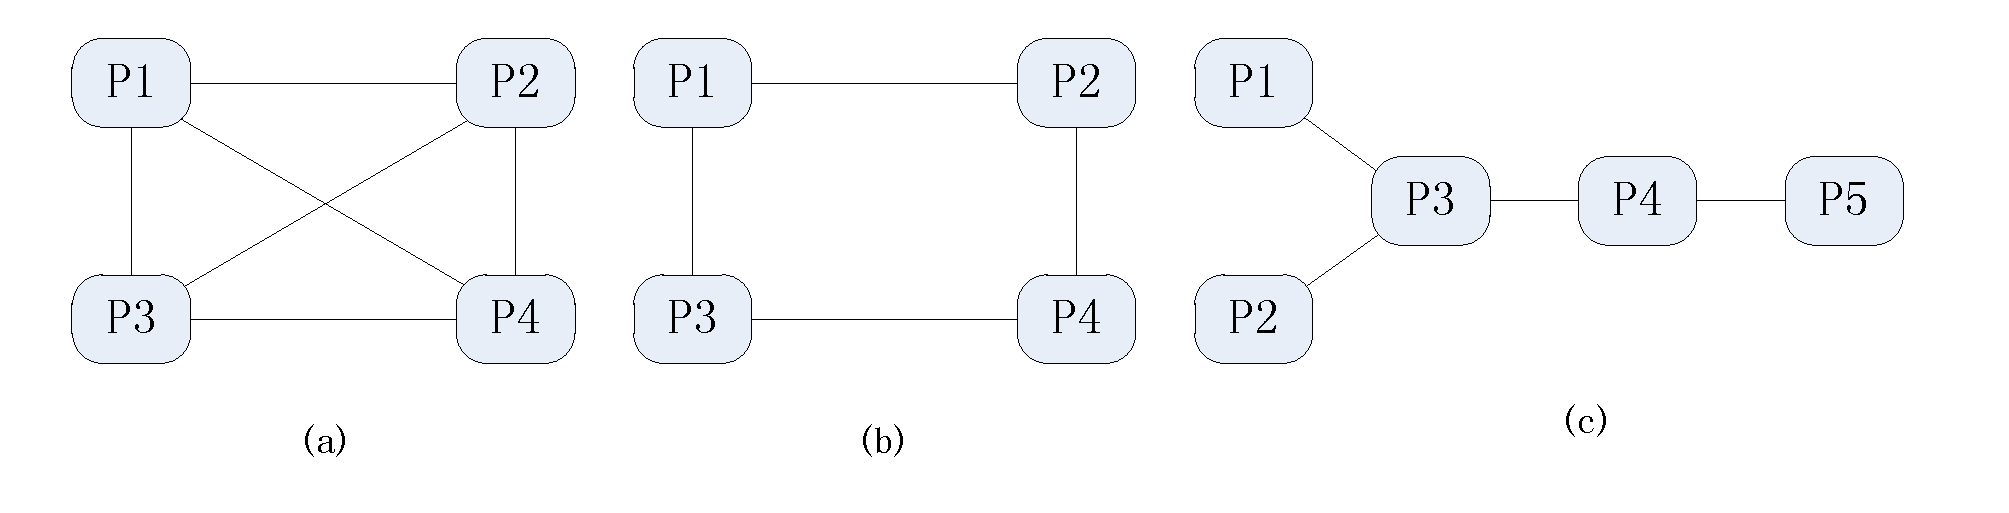
\includegraphics[height=17ex]{figure/DLS-p-connect.pdf}\\
  \caption{处理器连接示例}\label{DLS-fig-connect}
\end{figure}

本文假定直接相连的处理器之间具有相同的数据传输速率。没有链路直接相连的处理器之间在传输消息时需要通过其他处理器间接传递,消息的路由由平台本身给出。为输入方便,本文假定处理器之间消息的传递是静态路由,即具有相同起点和终点的消息通过相同的路径传递,消息传递选择具有最小跳数的路径。处理器间的路由信息由下一跳矩阵 H 给出,矩阵中 $H_{ij}$  表示当消息从处理器 i 要发往 j 时,要将其发往 $H_{ij}$ 号处理器。如下矩阵 $H_2$ 给出了图 \ref{DLS-fig-connect} 中 (b) 连接情况下的一种下一跳矩阵。

\begin{equation*}
  H_2=\begin{bmatrix}
      -1 & 2 & 3 & 2 \\
      1 & -1 & 1 & 4 \\
      1 & 1 & -1 & 4 \\
      2 & 2 & 3 & -1
  \end{bmatrix}
\end{equation*}

例如要从 1 号处理器发消息给 4 号处理器,由于没有链路直接相连,矩阵中 $H_{14}=2$ 表示先将消息发往 2 号处理器,再查看 $H_{24}=4$ 表示可直接从2 号处理器发往 4 号处理器。


根据 \ref{basic-partition} 节的描述,分区是分区操作系统分配资源的单位,任务单独运行于一个分区中,运行环境由分区所提供的资源来保证。分区系统对各分区之间的隔离性,保证了运行于不同分区中的任务不会相互影响。为了保证任务之间的隔离,在每个处理器中我们将任务与分区一一对应,其三者间的关系如图 \ref{DLS-fig-task-partition-relation}所示,图中表示4个处理器组成的环状网络以及其中的分区与任务对应关系。

\begin{figure}[!hbt]
  \centering
  % Requires \usepackage{graphicx}
  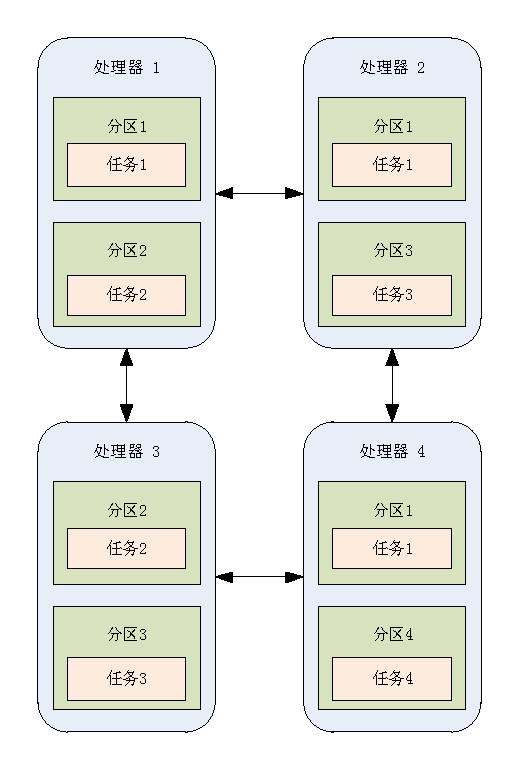
\includegraphics[height=60ex]{figure/DLS-task-partition-relation.pdf}\\
  \caption{处理器、分区和任务之间的关系}\label{DLS-fig-task-partition-relation}
\end{figure}

如在处理器 1 上,任务 $t_1$ 运行于分区1,我们在调度时为分区1分配的处理器时间分片的长度直接取决于其中运行的任务 $t_1$ 需要的运行时间,即 $t_1$ 的最坏运行时间 $C_1$。 这样,多核分区系统中对任务的调度,就转化为对分区的调度。由于每个任务的时间属性和任务之间的数据传输关系在调度前是已知的,我们就可以在系统运行前确定每个分区需要多少处理器时间,分别从哪个时刻开始到哪个时刻结束,这就是本文调度算法最后生成的针对每个处理器的任务调度表,同时也是每个处理器上的分区调度表。根据以上所述分区与任务间的一一对应关系,本文以下叙述中将不严格区分任务与分区的概念。

关于分区间的通信,如\ref{basic-partition-message}节所述,本文此处假定处于同一处理器的分区之间通信延迟可忽略,而不同处理器的分区间通信延迟与数据量和处理器之间的传输速率相关,在通信链路空闲的情况下,传递 M 的数据会造成 $M/s$ 的时间延迟。此外,本文将消息传递的距离也加入考虑:传递同样的数据量,随着消息跳数的增加,会稍稍增加传递延迟,使得跳数少的处理器结点被优先选择。
%\section{路由策略}
%
%在 \ref{basic-DAG-sch} 一节中介绍了 DAG 调度问题的几个分类,其中考虑处理器或核间消息路由的主要是 APN 类问题。在针对 APN 类问题的算法中,关注点主要集中于任务分配的顺序和任务向哪个处理器核心调度,至于消息路由则需要用户提供。因此在从DAG生成调度表时,首先也需要考虑了目标处理器平台的路由选择问题。%这里我们假定所有直接相连的核间通信的传输速率一致,也即相邻核间传输同样数据所花费的时间相同,这样,多核连接的拓扑结构就相当于一个边权值相等或无权的无向图。我们的路由选择策略总是选择路程最短,也即经过核数最少的路径。
%
%\subsection{静态路由}
%目标平台中,消息从一个核心发往另一个核心,对于静态路由来说,如果相同起点和终点,每次都选择同样的路径。最容易想到的,就是直接选择从起点到终点的最短路径。为简单起见,假定相邻(有链路直接相连的)处理器核心之间的数据传输速率都相同,那么目标处理器平台即成为一个无权无向连通图,处理器为顶点,链路为边,且所有边的权值都是1。在这个图上静态路由问题就化归为求解无权图任意顶点对之间的最短路径问题。假设图中顶点数为V,从图中一个顶点到达所有其他顶点的最短路径可以用一次广度优先顺序遍历得到,其复杂度为O$(V)$,那么求解所有顶点对之间最短路径的复杂度就是O$(V^2)$。
%
%静态路由的优点是路由信息可以事先计算,且算法实现方便。它的缺点在于不能根据消息在链路中的分布选择其他可以更早到达目标处理器核心的路径,这在非对称的处理器平台上有可能造成枢纽部分链路的消息过度密集而外围消息分布稀疏。
%
%\subsection{动态路由}
%
%动态路由在不同时刻从同一起点发往同一终点的消息可以选择不同的路径,其路径是在消息需要发送时才计算的,可以根据当时已调度消息在链路中的分布动态决定走哪条路径最快。这里的``快''指的是消息可以最早到达目标处理器核心,因此选择路径时势必要考虑不能覆盖所有可能链路上已分配的其他消息。
%
%即使是在无权连通图上,每次寻找从起点到终点的过程仍然是一个类似最短路问题中 Dijkstra 算法的过程,其复杂度为 O$(V\log{V})$,且在多次查找中仍需要针对同一起点和终点反复进行这一过程,大大提高了路由算法的开销,这是动态路由策略的一个劣势,开销较大、实现复杂。其优势是有可能找到更早到达的消息路由,使其后运行的任务有可能提前。但由于动态路由从路径上来说不一定是最短的,多次绕远路的消息路径有可能带来系统整体通信过大,也有造成原本可以更早调度的消息被多出来的通信开销给推后的结果。
%
%综合考虑以上两种路由策略的优劣,本文选择静态路由策略来实现算法。

% 路由算法描述:寻找最短路、生成下一跳矩阵





\section{任务分配}

本节首先假定任务调度是非抢占的,后面再对抢占式调度给出解决方案。

\subsection{任务排序与算法选择}

% DLS 最小松弛时间优先
% MH  最早时间限优先(未考虑不同任务可能由于约束条件 开始时间不同)
% 因此 DLS > MH

在\ref{basic-DAG-sch}一节中简要介绍了现有的几类 DAG 调度问题及其对应的算法。除了个别特殊条件下,DAG 调度本身几乎都是 NP 完全问题\upcite{DAGNP},在考虑数据通信的条件下,更进一步加大了问题的复杂性。文章 \cite{Comparison} 比较了解决 APN 问题的几种算法,并对不同条件下的调度结果做出了比较。% 描述优劣选择依据
%综合考虑调度优劣、算法本身的流程与我们这里所要解决问题的特殊性(虚拟结点的处理),我们选择 DLS 算法\upcite{DLS} 作为从 DAG 构建静态调度表的基础算法。

下面结合当前问题考虑相关算法的优劣。MH 算法\upcite{MHScheduling}根据 DAG 中每个结点的静态层数 (SBL) 属性排序,从大到小依次分配。由于 SBL 反映了该结点后面最少还有多少任务需要调度,SBL 越大说明任务需要越早完成。因此 MH 算法相当于单处理器实时调度中 EDF 算法的思想,时间限越早的任务具有更高的优先级。Dynamic Level Scheduling (DLS) 算法\upcite{DLS}则使用了一个动态层次 DL(Dynamic Level)作为排序标准。DL 是一个结点的 SBL 与它在一个处理器核心上的最早开始时间之差,具有最大 DL 的 (结点-核心) 对被挑选出来进行调度。这个值反映了该任务在满足时间限的前提下还有多大的调度空余度,相当于单处理器实时调度中最短空闲时间优先 (LLF) 算法的思想。

考虑在含有优先关系的多核调度环境下,不同任务由于制约条件不同,即使都处在可以运行的状态,能够开始的最早时间也可能不同。DLS 算法同时考虑了任务的开始与结束时间,而 MH 仅考虑任务的结束时间,这在所有就绪任务的最早开始时间不同的情况下未全面考虑所有因素。因此认为在当前问题的环境下,调度效果上 DLS 应当是优于 MH 算法的。

此外,如\ref{basic-DAG-sch}节所述,解决 DAG 调度 APN 问题的还有 BU 和 BSA 算法。这两类算法都是针对 DAG 调度问题的特点,首先将所有任务调度到枢轴处理器上去,再渐渐优化为更好的调度序列。但 DAG 调度问题不受虚拟任务结点的约束,在优化的过程中每一步都是一种可行调度方案,而在本文的 DAG 中,虚拟结点关于时间和连续调度的约束使得不能简单的将所有任务调度到一个处理器上,因此这两个算法都不太适合本文所述的情况。

综上所述,本文在此步骤中考虑使用 DLS 算法作为调度框架。

DLS 算法在调度的过程中,对就绪池中的每个结点,计算它们在所有处理器核心上的 DL,具有最大 DL 的 (结点- 核心) 对被挑选出来进行调度。其中在考虑各个任务于每个核心上的最早开始时间时,需要根据上一节提到的路由策略来决定,并同时记录下达到此开始时间时消息在链路上的调度信息。

% 为何不选用 BSA 。。。

\subsection{处理器排序}
\label{DLS-processor-sort}

% 来自 BSA 算法的思想,说明好处
% 最好有实验结果说明有必要对处理器核心排序

在将任务向处理器分配时,需要按一定顺序依次尝试将任务调度到各个处理器上。当某个任务在多个处理器上都具有相同的开始时间时,任务将被更优先于分配到排在前面的处理器上,因此,尝试分配的顺序对最终结果也会产生一定影响。如果排在前面的都是分布比较边缘的处理器,任务在目标平台上的分布也易分布于边缘,而边缘区处理器间连接数较少,造成通信路径比较长,整体通信开销变大。

我们借鉴 BSA 算法\upcite{BSA} 中任务分配顺序的思路,如果按照每个处理器的连接数从大到小排序,任务将更倾向于被分配到目标处理器平台的中枢地区,处理器间连接比较充分,之间的消息通信也比较通畅,使得整体系统通信开销减小。

\subsection{调度策略}

% 按时间段的查找方式分为
% 抢占、非抢占 两种

最终需要针对每个处理器核心,和每条链路都生成一个调度表。当需要将新任务加入某个处理器核心,或是将新消息加入对应链路上的消息调度表时,可以抢占或非抢占两种方式处理。如果是非抢占式调度,根据新添加任务所需的运行时间,需要在调度表中找到一块足够长的时间段将其分配给新任务;而对于抢占式调度,只需将任务按照时间限制尽早开始即可,如果一个时间段不够,则顺延至调度表的下一个时间段继续执行。

抢占与非抢占式调度在时间上的一大区别是,非抢占式调度根据任务的开始时间即可明确知道任务会在何时结束,而抢占式调度任务开始的早晚与任务结束的早晚并没有必然联系。这样,处理抢占式任务时,在以上 MDLS 算法中,在寻找 (任务-核心) 对时,需要将任务的最早开始时间改为考虑任务的最早完成时间,其他按原算法处理即可。

\section{虚拟结点}
\label{DLS-virtual-node}

DAG中的虚拟结点的处理需要考虑以下两个方面:
\begin{itemize}
  \item 它们不应当被分配到正常的处理器上去,否则将占用CPU 资源,延误普通任务的执行
  \item 它们和其他任务之间的通信数据不应当占用通信开销,因为所有数据也都是虚拟的,只用于表示先后依赖关系,并没有真正的数据流通。
\end{itemize}

可以在系统中加入一个虚拟分区专门用来分配虚拟任务。该分区与其他所有分区直接相连,且数据在与虚拟分区的链路传输不耗费时间。

在处理每个结点时,需要判断是否是虚拟结点,如果是则将其分配至虚拟处理器核心。根据 \ref{SDF-time-constraint} 一节所述,如果虚拟任务可以在虚拟处理器上连续分布,则所有任务的时间限都得到满足;否则,必有任务的时间限无法得到满足,调度失败。

\section{修改的DLS算法}
\subsection{算法流程}
综合考虑以上几节所讨论的问题,本文提出了修改的 DLS (Modified DLS, MDLS) 算法如算法 \ref{algo-MDLS} 所述。
\begin{algorithm}
  \caption{Modified DLS 算法}
  \label{algo-MDLS}
  \KwIn{包含虚拟结点的 DAG 任务图,目标处理器平台}
  \KwOut{任务和消息的静态调度表}
  向目标平台添加虚拟处理器\;
  将所有处理器按连接数降序排列\;
  计算 DAG 中所有结点的 SBL\;
  建立 ReadyTask 集合 S,并加入所有就绪结点\;
  \While{S 不空}{
      \uIf{S中有虚拟结点}{
          将结点尽可能早的调度至虚拟处理器\;
          \If{虚拟结点与前一个任务间有时间间隙}{
              无法得到有效调度\;
              算法结束\;
          }
      }\Else{
          考察 S 中所有任务与核组成的(任务-核)对,选择能够最早开始的任务,将其调度到对应的处理器上去\;
      }
  }
  更新 S 集合\;
\end{algorithm}

%\begin{Verbatim}[numbers=left,frame=single,xleftmargin=50pt]
%向目标平台添加虚拟处理器
%将所有处理器按连接数降序排列
%计算 DAG 中所有结点的 SBL
%建立 ReadyTask 集合 S,并加入所有就绪结点
%WHILE S不空 DO
%    IF S中有虚拟结点 THEN
%        将结点尽可能早的调度至虚拟处理器
%        IF 虚拟结点与前一个任务间有时间间隙 THEN
%            无法得到有效调度
%            算法结束
%        END IF
%    ELSE
%        考察S中所有任务与核组成的(任务-核)对,
%          选择能够最早开始的任务,将其调度到对
%          应的处理器上去
%    END IF
%    更新 S 集合
%END WHILE
%\end{Verbatim}

这样,即可得到目标平台每个处理器上的静态调度表,以及对应链路上的消息调度。

\subsection{复杂度分析}
\label{COSS-complexity}
假设 DAG 中结点个数为 $V_D$,目标平台处理器或核心数为 m。在上述算法过程中,对处理器按连接数降序排列的时间复杂度为 $O(m\log{}m)$,计算所有结点的 SBL 可由一遍深度优先遍历来完成,因此时间复杂度为 $O(V_D)$。

根据 \ref{basic-DLS-intro} 节的介绍可知,DLS 算法的时间复杂度为 $O({V_D}^{2}m f(m))$。与之相比,我们在 DLS 算法的循环内部添加了一个对虚拟结点的判断过程,该过程自身是$O(1)$的,而循环是对每个结点进行,因此与原 DLS 算法相比,总体多了一个 $O(V_D)$ 的过程。模型假设目标平台是静态路由,$f(m)=m$。

综上可知,对 MDLS 算法来说,总的复杂度为 $$O(m\log{}m)+O(V_D)+O({V_D}^{2}m^2)+O(V_D)=O({V_D}^{2}m^2)$$

再结合前两章中复杂度的分析,得到 COSS 算法总的复杂度为
$$O(V_G+E_G)+O(E_G+V_G+E_D+V_D)+O({V_D}^{2}m^2)=O(E_G+V_G+E_D+{V_D}^{2}m^2)$$
从 GSDF 到 DAG 的转换中,GSDF 中的每个结点都至少在 DAG 中出现一次,因此 $V_D\geqslant{}V_G$,对边来说也有类似关系 $E_D\geqslant{}E_G$,而 DAG 中边数最多为 $O({V_D}^2)$ 量级,因此上式可进一步化简为$$O({V_D}^{2}m^2)$$ 此即为 COSS 算法总的时间复杂度。

\section{本章小结}

本章设计了 COSS 算法的第三步,论述了从 DAG 求得静态调度表时所遇到目标平台抽象、任务分配和虚拟结点的处理等几个问题,针对每一问题分别讨论了可行方案及算法选择,最终提出了 MDLS 算法并给出了详细的描述。通过本章所述内容,COSS 算法主体部分结束,结合前两章,即可实现周期性任务集从时间、通信约束到目标平台的静态调度表。


